% ===== CHAPTER 10 =====
\chapter{电子自旋和自旋-统计定理}
\label{chap:10}
\section{电子自旋}
\label{sec:10.1 Electron Spin}

    所有化学家都熟悉钠原子在火焰中呈现的黄色。事实上,钠原子光谱中最强的黄色线(D线)是两条间隔很近的线。钠的D谱线由激发态$1s^22s^22p^63p$到基态的跃迁产生。\ce{Na} 光谱中这条线和其他线的双线性质表明,价电子可用的预期状态数增加了一倍。

    为了解释原子光谱的这种微观结构,Uhlenbeck 和 Goudsmit 于 1925 年提出,除了电子围绕原子核运动所产生的轨道角动量之外,电子还具有一种\textit{内禀}(内在)角动量。如果我们把电子想象成一个围绕其直径之一旋转的电荷球,我们就能明白这种内禀角动量是如何产生的。因此,我们得到了术语\textbf{自旋角动量}(spin angular momentum),或更简单地,\textbf{自旋}(spin)。然而,电子 “自旋”并不是一种经典效应,电子绕轴旋转的图景并不符合物理现实。内禀角动量是真实存在的,但没有一个容易又直观的模型能够正确解释它的起源。我们不能指望根据宏观世界的经验来理解微观粒子。除了电子,其他基本粒子也有自旋角动量。

    1928 年,狄拉克提出了电子相对论量子力学,在他的研究中,电子自旋自然而然地产生了。

    在我们所局限的非相对论量子力学中,电子自旋必须作为附加假设引入。我们已经了解到,在量子力学中,每种物理属性都有其对应的线性厄米算符。对于轨道角动量等性质,我们可以用相应的算符代替 $p_x$、$p_y$和$p_z$,从经典表达式中构造出量子力学算符。微观粒子固有的自旋角动量在经典力学中没有类似的表达式,因此我们不能用这种方法来构造自旋的算符。为了我们的目的,我们将只使用符号来表示自旋算符,而不给出它们的明确形式。

    与轨道角动量算符$\hat{L}^2, \hat{L}_x, \hat{L}_y, \hat{L}_z$类似,自旋算符也有对应的形式$\hat{S}^2, \hat{S}_x, \hat{S}_y, \hat{S}_z$,假设它们是线性厄米算符。$\hat{S}^2$ 是粒子总自旋角动量大小平方的算符。$\hat{S}_z$ 是自旋角动量在 $z$ 方向上的分量算符。我们有
    \begin{equation}
        \hat{S}^2 = \hat{S}_x^2 + \hat{S}_y^2 + \hat{S}_z^2.
        \label{eq:10.1}
    \end{equation}
    假设自旋角动量算符遵循轨道角动量算符相同的对易关系。与$\left[\hat{L}_x, \hat{L}_y\right] = \mathrm{i} \hbar \hat{L}_z$,$\left[\hat{L}_y, \hat{L}_z\right] = \mathrm{i} \hbar \hat{L}_x$,$\left[\hat{L}_z, \hat{L}_x\right] = \mathrm{i} \hbar \hat{L}_y$[式(\ref{eq:5.46})和(\ref{eq:5.48})],我们有
    \begin{equation}
        \left[\hat{S}_x, \hat{S}_y\right] = \mathrm{i} \hbar \hat{S}_z, \quad
        \left[\hat{S}_y, \hat{S}_z\right] = \mathrm{i} \hbar \hat{S}_x, \quad
        \left[\hat{S}_z, \hat{S}_x\right] = \mathrm{i} \hbar \hat{S}_y.
        \label{eq:10.2}
    \end{equation}
    根据(\ref{eq:10.1})和(\ref{eq:10.2}),通过求得(\ref{eq:5.49})和(\ref{eq:5.50})时所用的算符代数,可以得出
    \begin{equation}
        \left[\hat{S}^2, \hat{S}_x\right] = \left[\hat{S}^2, \hat{S}_y\right] = \left[\hat{S}^2, \hat{S}_z\right] = 0
        \label{eq:10.3}
    \end{equation}
    由于公式 (\ref{eq:10.1}) 和 (\ref{eq:10.2}) 是公式 (\ref{eq:5.107}) 和 (\ref{eq:5.108}) 的形式,根据第 \ref{sec:5.4 The Ladder-Operator Method for Angular Momentum} 节的工作(只取决于对易关系,而不取决于算符的具体形式),可以得出 $\hat{S}^2$ 的本征值为[式(\ref{eq:5.142})]
    \begin{equation}
        \boxed{
            s\left(s+1\right)\hbar^2, \quad s = 0, \frac{1}{2}, 1, \frac{3}{2}, \ldots
        }
        \label{eq:10.4}
    \end{equation}
    以及$\hat{S}_z$ 的本征值为[式(\ref{eq:5.141})]
    \begin{equation}
        \boxed{
            m_s\hbar, \quad m_s = -s, -s+1, \ldots, s-1, s
        }
        \label{eq:10.5}
    \end{equation}

    量子数$s$称为粒子的\textbf{自旋量子数}(spin quantum number)。尽管第 \ref{sec:5.4 The Ladder-Operator Method for Angular Momentum} 节中并没有限制电子的 $s$ 值只能是单一的,但实验表明,所有电子的 $s$ 值都是单一的,即$s = \frac{1}{2}$。质子和中子同样有$s = \frac{1}{2}$。离子有$s = 0$。光子则有$s=1$。然而,公式 (\ref{eq:10.5}) 对光子并不成立。光子在真空中以 $c$ 的速度传播。由于其相对论性质,光子可以有以下两种情况:$m_s = +1$ 或 $m_s = -1$,但不具有$m_s = 0$(见\textit{Merzbacher}, Chapter 22)。这两个 $m_s$ 值分别对应左旋圆偏振光和右旋圆偏振光。

    有了$s = \frac{1}{2}$,电子总自旋角动量的值由(\ref{eq:10.4})的平方根给出:
    \begin{equation}
        \left[\frac{1}{2}\left(\frac{3}{2}\right)\hbar^2\right]^{1/2}=\frac{1}{2}\sqrt{3}\hbar
        \label{eq:10.6}
    \end{equation}
    对于$s = \frac{1}{2}$,式(\ref{eq:10.5})给出了电子$\hat{S}_z$的可能本征值为$+ \frac{1}{2}\hbar$和$-\frac{1}{2}\hbar$。因对应于这些$\hat{S}_z$本征值的电子自旋本征函数由$\alpha$和$\beta$给出:
    \begin{equation}
        \boxed{
            \hat{S}_z \alpha = + \frac{1}{2}\hbar \alpha
        }
        \label{eq:10.7}
    \end{equation}
    \begin{equation}
        \boxed{
            \hat{S}_z \beta = - \frac{1}{2}\hbar \beta
        }
        \label{eq:10.8}
    \end{equation}
    由于$\hat{S}_z$和$\hat{S}^2$可对易,我们可以将$\hat{S}_z$的本征函数变为$\hat{S}^2$的本征函数,有了$s = \frac{1}{2}$和(\ref{eq:10.4})给出的本征值,我们有
    \begin{equation}
        \hat{S}^2 \alpha = \frac{3}{4}\hbar^2 \alpha, \quad
        \hat{S}^2 \beta = \frac{3}{4}\hbar^2 \beta
        \label{eq:10.9}
    \end{equation}
    $\hat{S}_z$和$\hat{S}_x$、$\hat{S}_y$不可对易,所以$\alpha$和$\beta$不是$\hat{S}_x$和$\hat{S}_y$的本征函数。术语\textit{自旋向上}(spin up)和\textit{自旋向下}(spin down)分别指的是$m_s = +\frac{1}{2}$和$m_s = -\frac{1}{2}$。见图10.1。稍后我们将证明,量子数 $m_s$ 的两种可能性会使碱金属光谱中的谱线条数加倍。
    \begin{figure}[ht]
        \centering
        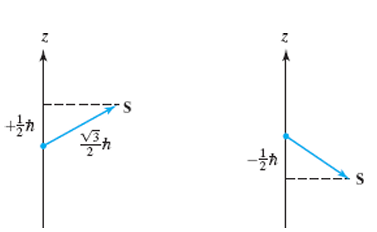
\includegraphics[width=0.4\textwidth]{Figures/10.1.png}
        \caption{
            \centering
            \parbox{\linewidth}{
                \centering 
                电子自旋矢量相对于 $z$ 轴的可能方向。在每种\\
                情况下,$\mathbf{S}$ 都位于以 $z$ 轴为轴的圆锥表面上。
            }
        }
        \label{fig:10.1}
    \end{figure}

    我们之前讨论过的波函数是粒子空间坐标的函数:$\psi = \psi\left(x,y,z\right)$。我们可能想问:自旋本征函数$\alpha$和$\beta$的变量是什么呢?有时,人们在谈论自旋坐标 $\omega$ 时,并没有明确说明这个坐标是什么。通常情况下,人们把自旋量子数 $m_s$ 作为自旋特征函数所依赖的变量。与空间波函数相比,这种程序很不寻常;但因为我们只有两种可能的电子自旋特征函数和本征值,所以这是一种方便的选择。我们有
    \begin{equation}
        \alpha = \alpha\left(m_s\right), \quad
        \beta = \beta\left(m_s\right)
        \label{eq:10.10}
    \end{equation}

    像往常一样,我们希望对本征函数进行归一化处理。单粒子空间波函数的三个变量范围在$-\infty$到$+\infty$之间连续变化,则归一化条件意味着
    \begin{equation*}
        \int_{-\infty}^{\infty} \int_{-\infty}^{\infty} \int_{-\infty}^{\infty} \left|\psi\left(x, y, z\right)\right|^2\: \mathrm{d}x\: \mathrm{d}y\: \mathrm{d}z = 1
    \end{equation*}
    电子自旋本征函数的变量 $m_s$ 只有 $+\frac{1}{2}$ 和 $-\frac{1}{2}$ 两个离散值。因此,对单粒子自旋本征函数的归一化意味着
    \begin{equation}
        \sum_{m_{s}=-1/2}^{1/2} \left|\alpha \left(m_{s}\right)\right|^{2} = 1, \quad \sum_{m_{s}=-1/2}^{1/2} \left|\beta \left(m_{s}\right)\right|^{2} = 1
        \label{eq:10.11}
    \end{equation}
    因为本征函数$\alpha$和$\beta$对应于厄米算符$\hat{S}_z$的不同本征值,所以它们是正交的:
    \begin{equation}
        \sum_{m_{s}=-1/2}^{1/2} \alpha^ * \left(m_{s}\right) \beta \left(m_{s}\right) = 0
        \label{eq:10.12}
    \end{equation}
    令$\alpha\left(m_s\right) = \delta_{m_s, 1/2}$,$\beta\left(m_s\right) = \delta_{m_s, -1/2}$,其中$\delta_{jk}$是Kronecker $\delta$函数,我们就满足了(\ref{eq:10.11})和(\ref{eq:10.12})。

    当我们考虑电子的完全波函数(包括空间和自旋变量)时,我们将根据以下公式对其进行归一化处理
    \begin{equation}
        \boxed{
            \sum_{m_s=-1/2}^{1/2} \int_{-\infty}^{\infty} \int_{-\infty}^{\infty} \int_{-\infty}^{\infty} \left|\psi\left(x, y, z, m_s\right)\right|^2 \:\mathrm{d}x \:\mathrm{d}y \:\mathrm{d}z = 1
        }
        \label{eq:10.13}
    \end{equation}
    符号
    \begin{equation*}
        \int \left|\psi\left(x, y, z, m_s\right)\right|^2 \:\mathrm{d}\tau
    \end{equation*}
    表示对自旋变量求和,对空间变量全范围积分,如 (\ref{eq:10.13}) 所示。符号 $\int \:\mathrm{d}v$ 表示对系统空间变量全范围的积分。

    \begin{quote}
        \small
        \noindent
        电子目前被认为是一种没有子结构的点状基本粒子。高能电子-正电子碰撞实验表明,没有证据表明电子的大小不为零,并将电子半径的上限为$3 \times 10^{-19} \:\mathrm{m}$[D. Bourilkov, \textit{Phys. Rev. D}, \textbf{62}, 076005 (2020); \url{arxiv.org/abs/hep-ph/0002172}.]。质子和中子是由夸克构成的,因此不是基本粒子。质子的均方根电荷半径为$0.88 \times 10^{-15} \:\mathrm{m}$。
    \end{quote}

\section{自旋和氢原子}
\label{sec:10.2 Spin and the Hydrogen Atom}

    具体说明电子状态的波函数不仅取决于$x$、$y$和$z$坐标,还取决于电子的自旋状态。这对氢原子的波函数和能级有什么影响?

    在很好的近似条件下,电子系统的哈密顿算符不涉及自旋变量,而只是空间坐标和关于空间坐标的导数的函数。因此,我们可以将单个电子的定态波函数分离为空间和自旋部分的乘积:
    \begin{equation*}
        \psi\left(x,y,z\right)g\left(m_s\right)
    \end{equation*}
    其中的$g\left(m_s\right)$是$\alpha$或$\beta$的其中之一,取决于$m_s = +\frac{1}{2}$或$m_s = -\frac{1}{2}$。[更一般地,$g\left(m_s\right)$可以是$\alpha$和$\beta$的线性组合;$g\left(m_s\right) = c_1 \alpha + c_2\beta$。]由于哈密顿算符对自旋波函数没有作用,我们有
    \begin{equation*}
        \hat{H} \left[\psi\left(x, y, z\right) g\left(m_s\right)\right] = g\left(m_s\right) \hat{H} \psi\left(x, y, z\right) = E \left[\psi\left(x, y, z\right) g\left(m_s\right)\right]
    \end{equation*}
    我们得到了与之前未考虑自旋时相同的能量。引入自旋唯一的不同是使得可能的状态数翻倍。与状态$\psi\left(x, y, z\right)$不同,我们有两个可能的状态$\psi\left(x, y, z\right) \alpha$和$\psi\left(x, y, z\right) \beta$。当我们考虑自旋时,氢原子能级的简并度是$2n^2$而不是$n^2$。

\section{自旋-统计定理}
\label{sec:10.3 Spin-Statistics Theorem}

    假设我们有一个由多个全同粒子组成的系统。在经典力学中,粒子的全同性不会导致特殊的后果。例如,考虑一下在台球桌上滚动的完全相同的台球。我们可以跟踪任何一个球的运动,比如通过拍摄系统的运动图像。我们可以说,一号球沿着某条轨迹运动,二号球沿着另一条确定的轨迹运动,以此类推,这些轨迹是由牛顿运动定律决定的。因此,虽然这些球是相同的,但我们可以通过指定每个球的运动轨迹来区分它们。球的特性对它们的运动没有特殊的影响。

    在量子力学中,不确定性原理告诉我们,我们无法追踪微观“粒子”的确切路径。如果系统中的微观粒子都具有不同的质量、电荷或自旋,我们就可以利用其中的一个特性来区分粒子。但如果它们都是相同的,那么我们在经典力学中区分它们的一种方法——即指定它们的路径——在量子力学中就会因为不确定性原理而丧失。因此,由相互作用的全同粒子组成的系统的波函数一定无法区分不同的粒子。例如,在第\ref{chap:9}章微扰理论处理氦原子激发态时,我们看见函数$1s\left(1\right)2s\left(2\right)$(说明电子1在$1s$轨道而电子2在$2s$轨道)不是一个正确的零级波函数。相反地,我们不得不使用函数$2^{-1/2}\left[1s\left(1\right)2s\left(2\right) \pm 1s\left(2\right)2s\left(1\right)\right]$,它无法指明电子在哪个轨道上。(如果相同的粒子彼此分离得很好,使它们的波函数不重叠,它们就可以被视为是可区分的。)

    现在,我们来推导量子力学中全同粒子的不可区分性对波函数的限制。由 $n$ 个相同微观粒子组成的系统的波函数取决于粒子的空间变量和自旋变量。对于粒子1,这些变量为$x_1$、$y_1$、$z_1$和$m_{s1}$。令$q_1$表示所有这四个变量。则$\psi = \psi\left(q_1, q_2, \ldots, q_n\right)$。

    我们定义交换两个粒子1和2所有坐标的算符$\hat{P}_{12}$为\textbf{交换算符}或\textbf{置换算符}(exchange or permutation operator):
    \begin{equation}
        \boxed{
            \hat{P}_{12} f\left(q_1, q_2, q_3, \ldots, q_n\right) = f\left(q_2, q_1, q_3, \ldots, q_n\right)
        }
        \label{eq:10.14}
    \end{equation}
    例如,对某表示电子1在$1s$轨道自旋向上而电子2在$3s$轨道自旋向下的函数,算符$\hat{P}_{12}$的作用为
    \begin{equation}
        \hat{P}_{12}\left[1s\left(1\right)\alpha\left(1\right)3s\left(2\right)\beta\left(2\right)\right] = 1s\left(2\right)\alpha\left(2\right)3s\left(1\right)\beta\left(1\right)
        \label{eq:10.15}
    \end{equation}

    $\hat{P}_{12}$的本征函数是什么?将$\hat{P}_{12}$作用两次,我们得到了原函数:
    \begin{equation*}
        \hat{P}_{12} \hat{P}_{12} f\left(q_1, q_2, \ldots, q_n\right) = \hat{P}_{12} f\left(q_2, q_1, \ldots, q_n\right) = f\left(q_1, q_2, ..., q_n\right)
    \end{equation*}
    因此,$\hat{P}_{12}^2 = \hat{1}$。设$\hat{P}_{12}$的本征函数和本征值分别为$w_i$和$c_i$。我们有$\hat{P}_{12} w_i = c_i w_i$。作用两次后,我们得到$\hat{P}_{12}^2 w_i = c_1 P_{12} w_i$。将$\hat{P}_{12}^2 = \hat{1}$和$\hat{P}_{12} w_i = c_i w_i$代入$\hat{P}_{12}^2 w_i = c_1 P_{12} w_i$,我们得到$w_i = c_i^2 w_i$。由于零不能作为本征函数,我们可以在两边同时除以$w_i$,得到$c_i^2 = 1$。因此,$c_i = \pm 1$。$\hat{P}_{12}$(以及任何平方为单位算符的线性算符)的本征值是$+1$和$-1$。

    若$w_+$是$\hat{P}_{12}$的本征函数,对应于本征值$+1$,则
    \begin{equation*}
        \hat{P}_{12}w_{+}\left(q_1, q_2, \ldots, q_n\right) = \left(+1\right)w_{+}\left(q_1, q_2, \ldots, q_n\right)
    \end{equation*}
    \begin{equation}
        \boxed{
            w_{+}\left(q_{2}, q_{1}, \ldots, q_{n}\right) = w_{+}\left(q_{1}, q_{2}, \ldots, q_{n}\right)
        }
        \label{eq:10.16}
    \end{equation}
    当粒子 1 和粒子 2 相互交换时,具有不变性质(\ref{eq:10.16})的函数(如 $w_+$)被称为与粒子 1 和粒子 2 相互交换\textbf{对称}(symmetric)的函数。对于本征值$-1$,我们有
    \begin{equation}
        \boxed{
            w_{-}\left(q_{2}, q_{1}, \ldots, q_{n}\right) = -w_{-}\left(q_{1}, q_{2}, \ldots, q_{n}\right)
        }
        \label{eq:10.17}
    \end{equation}
    (\ref{eq:10.17})的函数(如 $w_-$)被称为与粒子 1 和粒子 2 相互交换\textbf{反对称}(antisymmetric)的函数,这意味着将$w_-$乘以$-1$会得到交换后的函数。任意函数$f\left(q_1, q_2, \ldots, q_n\right)$对粒子1和2交换对称或是交换反对称无关紧要。

    不要混淆粒子互换的对称或非对称性质与空间反转的偶函数或奇函数性质。对于粒子1和2的交换,函数$x_1 + x_2$是交换对称的,它是$x_1$和$x_2$的奇函数。函数$x_1^2 + x_2^2$是交换对称的,但它是$x_1$和$x_2$的偶函数。

    算符$\hat{P}_{ik}$定义为
    \begin{equation}
        \hat{P}_{ik} f \left(q_1, \ldots, q_i, \ldots, q_k, \ldots, q_n\right) = f \left(q_1, \ldots, q_k, \ldots, q_i, \ldots, q_n\right)
        \label{eq:10.18}
    \end{equation}
    与$\hat{P}_{12}$类似,$\hat{P}_{ik}$的本征值为$+1$和$-1$。

    现在我们来看看由 $n$ 个相同的微观粒子组成的系统的波函数。由于粒子是无法区分的,我们给它们贴标签的方式不会影响系统的状态。因此,两个波函数
    \begin{equation*}
        \psi\left(q_1, \ldots, q_i, \ldots, q_k, \ldots, q_n\right) \quad \text{和} \quad \psi\left(q_1, \ldots, q_k, \ldots, q_i, \ldots, q_n\right)
    \end{equation*}
    必须对应于系统的相同状态。对应同一状态的两个波函数最多只能相差一个乘法常数。因此
    \begin{equation*}
        \begin{aligned}
            \psi\left(q_1, \ldots, q_k, \ldots, q_i, \ldots, q_n\right) &= c \psi\left(q_1, \ldots, q_i, \ldots, q_k, \ldots, q_n\right) \\
            \hat{P}_{ik} \psi\left(q_1, \ldots, q_i, \ldots, q_k, \ldots, q_n\right) &= c \psi\left(q_1, \ldots, q_i, \ldots, q_k, \ldots, q_n\right)
        \end{aligned}
    \end{equation*}
    最后一个方程表明$\psi$是算符$\hat{P}_{ik}$的本征函数。但是我们知道$\hat{P}_{ik}$的本征值只能是$+1$或$-1$。我们得出结论:由 $n$ 个全同粒子组成的系统,其波函数必须与任意两个全同粒子 $i$ 和 $k$ 的互换对称或反对称。由于 $n$ 个粒子都是相同的,我们不可能让波函数与某些互换对称,而与其他互换反对称。因此,$n$ 个完全相同的粒子的波函数必须要么与每一种可能的交换对称,要么与两个粒子的每一种可能的交换反对称。[刚才的论证并不严谨。完全相同的粒子系统的波函数对于两个粒子的互换必须是完全对称或完全反对称的说法称为\textit{对称化假设}(symmetrization postulate)。]

    我们已经看到,全同粒子系统的波函数有两种可能的情况,即对称和非对称情况。实验证据(如稍后讨论的元素周期表)表明,对于电子来说,只有反对称情况才会出现。因此,我们有了量子力学的另一个假设,即\textit{电子系统的波函数在任意两个电子互换时必须是反对称的}。

    1926 年,狄拉克根据理论研究和实验数据得出结论:电子要求反对称波函数,光子要求对称波函数。然而,狄拉克和其他物理学家在 1926 年错误地认为所有物质粒子都要求反对称波函数。1930 年,实验数据表明,$\alpha$ 粒子($s=0$)要求对称波函数;物理学家最终认识到,决定一个全同粒子系统要求对称波函数还是反对称波函数的是粒子的自旋性质。具有半整数自旋量子数($s = \frac{1}{2}, \frac{3}{2}$,等等)的粒子要求反对称波函数,而具有整数自旋量子数($s = 0, 1, 2$,等等)的粒子要求对称波函数。1940 年,物理学家沃尔夫冈·泡利(Wolfgang Pauli)利用相对论量子场论证明了这一结果。要求反对称波函数的粒子,如电子,被称为\textbf{费米子}(fermions)(以 E. Fermi 命名),而要求对称波函数的粒子,如离子,则被称为\textbf{玻色子}(bosons)(以 S. N. Bose 命名)。在非相对论量子力学中,我们必须假设,如果粒子具有半整数自旋量子数,则全同粒子系统的波函数在任意两个粒子互换时必须是反对称的;如果粒子具有整数自旋量子数,则波函数在互换时必须是对称的。这句话被称为\textbf{自旋-统计定理}(spin-statistics theorem)(因为玻色子系统的统计力学与费米子系统的统计力学不同)。

    自旋统计定理有许多不同有效性的证明;见 I. Duck and E. C. G. Sudurshan, \textit{Pauli and the Spin-Statistics Theorem}, World Scientific, 1997;\textit{Am. J. Phys.}, \textbf{66}, 284 (1998); Sudurshan and Duck, \textit{Pramana-J. Phys.}, \textbf{61}, 645 (2003) (见 \url{www.ias.ac.in/pramana/v61/p645/fulltext.pdf})。一些实验以极高的精度证实了自旋统计定理的有效性;见 G. M. Tino, \textit{Fortschr. Phys.}, \textbf{48}, 537 (2000) (可查阅 \url{arxiv.org/abs/quant-ph/9907028})。

    自旋-统计定理对完全相同的费米子系统有一个重要的影响。反对称要求意味着
    \begin{equation}
        \psi\left(q_1, q_2, q_3, \ldots, q_n\right) = -\psi\left(q_2, q_1, q_3, \ldots, q_n\right)
        \label{eq:10.19}
    \end{equation}
    考虑当电子1和2有相同坐标时$\psi$的值,即$x_1 = x_2$,$y_1 = y_2$,$z_1 = z_2$,$m_{s1} = m_{s2}$。在(\ref{eq:10.19})中令$q_2 = q_1$,我们得到
    \begin{equation*}
        \begin{aligned}
            \psi\left(q_1, q_1, q_3, \ldots, q_n\right) &= -\psi\left(q_1, q_1, q_3, \ldots, q_n\right) \\
            2\psi &= 0
        \end{aligned}
    \end{equation*}
    \begin{equation}
        \psi\left(q_1, q_1, q_3, \ldots, q_n\right) = 0
        \label{eq:10.20}
    \end{equation}
    因此,两个自旋相同的电子在三维空间的同一点出现的概率为零。(“自旋相同”意味着$m_s$值相等。)由于$\psi$是连续函数,方程(\ref{eq:10.20})说明在空间中发现两个自旋相同的电子彼此靠近的概率非常小。因此,反对称要求迫使自旋相同的电子彼此分开。为了描述这一点,人们常说这种电子之间存在\textbf{泡利斥力}(Pauli repulsion)。这种 “斥力”并不是一种真正的物理力,而是电子波函数在交换时必须是反对称的这一事实的反映。

    对称或反对称波函数的要求也适用于两个或多个全同复合粒子的系统。例如,考虑分子\ce{^16 O2}。\ce{^16 O}的核由8个质子和8个中子组成。每个质子和中子都满足$s = \frac{1}{2}$,都是费米子。因此,交换两个\ce{O}原子核相当于交换16个费米子的坐标,需要将分子的波函数乘以$\left(-1\right)^{16} = 1$。因此,分子\ce{^16 O2}的波函数在核坐标交换时是对称的。对相同原子核交换对称性或反对称性的要求会影响分子波函数的简并性,并导致转动配分函数中的对称数[见\textit{McQuarrie} (2000), pp. 104-105]。

    对于包含 $m$ 个全同玻色子和 $n$ 个全同费米子的两个相同复合粒子的交换,波函数需乘以$\left(+1\right)^m$\\$\left(-1\right)^n = \left(-1\right)^n$。

    因此,如果复合粒子包含奇数个费米子,那么它就是费米子,否则就是玻色子。

    当使用变分原理(第 \ref{sec:8.1 The Variation Theorem} 节)来获取原子和分子的近似电子波函数时,要求试探函数具有良好的稳定性,其中包括要求它具有反对称性。

\section{氦原子}
\label{sec:10.4 Th Helium Atom}



















\section{泡利不相容原理}
\label{sec:10.5 The Pauli Exclusion Principle}

\section{斯莱特行列式}
\label{sec:10.6 Slater Determinants}

\section{微扰理论处理基态锂原子}
\label{sec:10.7 Perturbation Treatment of the Lithium Ground State}

\section{变分法处理基态锂原子}
\label{sec:10.8 Variation Treatments of the Lithium Ground State}

\section{自旋磁矩}
\label{sec:10.9 Spin Magnetic Moment}

\section{电子自旋的梯度算符}
\label{sec:10.10 Ladder Operators for Electron Spin}

\section*{总结}

\section*{习题}